\chapter{Resultados Preliminares}
\label{cap:resultados}

Este capítulo apresenta os resultados iniciais obtidos com a implementação de um protótipo do \gls{agbo}, conforme descrito na Metodologia. O objetivo desta etapa preliminar é validar a corretude da implementação dos componentes do algoritmo e avaliar sua capacidade de convergência em um cenário controlado. Para isso, o protótipo foi aplicado a sete instâncias de grafos da classe dos completos ($K_n$), cujo valor de $\lambda(G)$ é dado por $2n - 2$ \cite{griggs1992labelling}, servindo como caso de teste ideal para a validação da abordagem.

\section{Implementação do Protótipo do AGBO}

O protótipo foi desenvolvido em \textit{Python}~3.12, utilizando as bibliotecas \texttt{NetworkX} para a criação, manipulação e serialização de grafos, \texttt{Matplotlib} para a geração de gráficos de convergência, \texttt{csv} para a exportação dos resultados em formato tabular e \texttt{concurrent.futures} para a execução paralela de múltiplas instâncias do algoritmo genético. A estrutura de dados dos grafos também foi convertida para o formato \texttt{json\_graph}, facilitando o intercâmbio entre processos.  
Os experimentos foram executados em um MacBook Air~M1, com 8~GB de memória RAM
e macOS 14.2.1 (Sonoma).  
Todas as dependências estão descritas no arquivo \texttt{requirements.txt} do
repositório de código, permitindo a reprodução dos resultados com o gerenciador
\texttt{pip}. O código-fonte completo encontra-se hospedado em um repositório público no
GitHub\footnote{\url{https://github.com/lazarguinho/agbo-l21} — acesso em:
15 jul. 2025}.

O operador de mutação adotado nesta etapa foi o \textit{Exchange Mutation} (\gls{em}), que atua trocando aleatoriamente dois genes da representação do indivíduo — neste caso, duas posições distintas da ordem dos vértices. Essa operação simples é suficiente para introduzir diversidade na população, permitindo a exploração de novas soluções viáveis sem violar a estrutura da representação.

\section{Experimento de Validação}

Para validar a implementação, foi conduzido um experimento em um conjunto de sete instâncias de grafos completos com número de vértices variando de 10 a 70, com incrementos de 10 vértices por instância. Esses grafos foram gerados aleatoriamente utilizando uma semente fixa para garantir a reprodutibilidade dos testes. Cada grafo \( K_n \) foi rotulado utilizando o protótipo do \gls{agbo}, configurado com com a seguinte configuração de parâmetros:

\begin{itemize}
    \item \textbf{Tamanho da população:} 20 indivíduos.
    \item \textbf{Número de gerações:} 100.
    \item \textbf{Taxa de mutação:} 10\% ($0.1$).
    \item \textbf{Operador de cruzamento:} \gls{cx}.
    \item \textbf{Operador de mutação:} \gls{em}.
\end{itemize}

Para cada instância, o algoritmo foi executado 5 vezes de forma independente, permitindo a avaliação de variabilidade no desempenho e a análise da capacidade de convergência. Os resultados de cada execução incluem: o menor \textit{span} encontrado, o tempo de execução, a melhor ordem dos vértices, a rotulação correspondente e o histórico de convergência. Os valores de \(\lambda(G)\) conhecidos para grafos completos \( K_n \) foram utilizados como referência para avaliar a qualidade das soluções encontradas. O Quadro~\ref{tab:resumo-kn} apresenta um resumo quantitativo com as estatísticas obtidas para cada instância, incluindo o número de vértices, o \textit{span} mínimo e médio, o tempo mínimo, médio e máximo, além do valor teórico de \(\lambda(G)\).

Além dos valores numéricos, foram gerados gráficos de convergência para cada execução, ilustrando a evolução do \textit{span} ao longo das gerações. Esses gráficos permitem observar o comportamento do algoritmo e sua estabilidade em relação a diferentes execuções sobre a mesma instância. A Figura~\ref{fig:convergencias-kn} apresenta uma seleção dessas curvas para fins ilustrativos.

\section{Análise Preliminar}

Os resultados preliminares são promissores e atingem o objetivo principal desta fase: \textbf{validar a corretude da implementação do AGBO}. O protótipo foi capaz de produzir rotulações–$L(2,1)$ em todas as instâncias testadas. Em todas as execuções, os valores de \textit{span} encontrados coincidiram com o valor ótimo teórico \(\lambda(G) = 2n - 2\), conforme esperado para grafos completos \(K_n\).

Não foi observada variação entre as execuções, o que indica estabilidade do algoritmo. Essa característica é reforçada pelas curvas de convergência apresentadas, que revelam uma linha reta constante no valor ótimo teórico desde as primeiras gerações. Isso demonstra que o algoritmo foi capaz de encontrar rapidamente soluções ótimas e mantê-las durante toda a execução, sem flutuações ou retrocessos. Esse padrão de convergência estável é particularmente esperado em grafos completos, cuja estrutura simétrica favorece a identificação precoce de rótulos ótimos.

O tempo de execução médio se manteve dentro de limites aceitáveis para o contexto de experimentação acadêmica, mesmo com a execução paralela de múltiplas instâncias. O desempenho escalonou de maneira proporcional ao tamanho dos grafos, como era de se esperar, e não foram observados gargalos computacionais durante os testes. Isso indica que a abordagem adotada, mesmo sendo um protótipo, é suficientemente eficiente para lidar com instâncias de pequeno e médio porte.

\begin{quadro}[htbp]
    \centering
    \caption{Resultados para grafos completos \(K_n\)}
    \label{tab:resumo-kn}
    \resizebox{\textwidth}{!}{
    \begin{tabular}{|c|c|c|c|c|c|c|c|}
        \hline
        \textbf{Grafo} & \(|V|\) & \textbf{Span mínimo} & \textbf{Span médio} & \(\lambda(G)\) & \textbf{Tempo min (s)} & \textbf{Tempo médio (s)} & \textbf{Tempo máx (s)} \\
        \hline
        \(K_{10}\) & 10 & 18 & 18.0 & 18 & 0.50 & 0.54 & 0.56 \\
        \(K_{20}\) & 20 & 38 & 38.0 & 38 & 5.18 & 5.26 & 5.34 \\
        \(K_{30}\) & 30 & 58 & 58.0 & 58 & 33.10 & 33.22 & 33.32 \\
        \(K_{40}\) & 40 & 78 & 78.0 & 78 & 100.92 & 101.68 & 102.16 \\
        \(K_{50}\) & 50 & 98 & 98.0 & 98 & 221.69 & 222.80 & 223.37 \\
        \(K_{60}\) & 60 & 118 & 118.0 & 118 & 433.69 & 436.31 & 438.77 \\
        \(K_{70}\) & 70 & 138 & 138.0 & 138 & 784.55 & 790.70 & 794.36 \\
        \hline
    \end{tabular}}
    \caption*{Fonte: Elaborado pelo autor.}
\end{quadro}


\begin{figure}[h]
    \centering
    \caption{Convergências das execuções}
    \label{fig:convergencias-kn}
    \resizebox{!}{0.5\textheight}{%
        \begin{minipage}{\textwidth}
            \begin{minipage}[b]{0.48\textwidth}
                \centering
                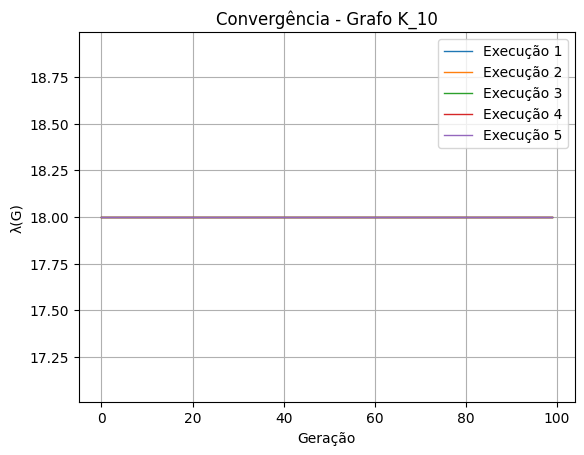
\includegraphics[width=\textwidth]{figuras/convergencia_1.png}
                \label{fig:convergencia-1}
            \end{minipage}
            \hfill
            \begin{minipage}[b]{0.48\textwidth}
                \centering
                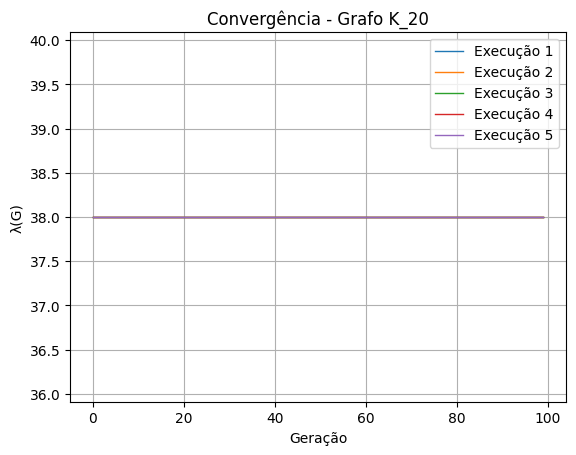
\includegraphics[width=\textwidth]{figuras/convergencia_2.png}
                \label{fig:convergencia-2}
            \end{minipage}
            
            \begin{minipage}[b]{0.48\textwidth}
                \centering
                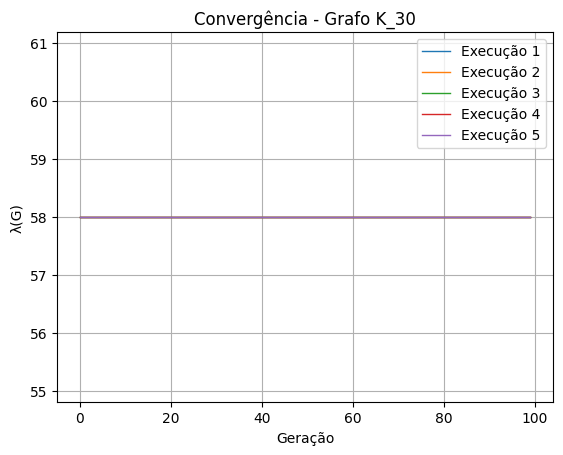
\includegraphics[width=\textwidth]{figuras/convergencia_3.png}
                \label{fig:convergencia-3}
            \end{minipage}
            \hfill
            \begin{minipage}[b]{0.48\textwidth}
                \centering
                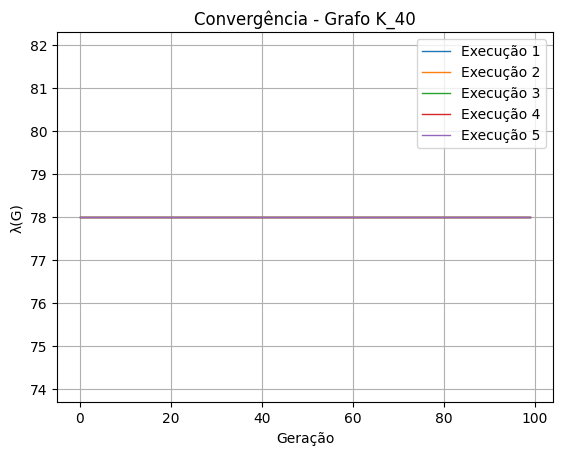
\includegraphics[width=\textwidth]{figuras/convergencia_4.png}
                \label{fig:convergencia-4}
            \end{minipage}
            
            \begin{minipage}[b]{0.48\textwidth}
                \centering
                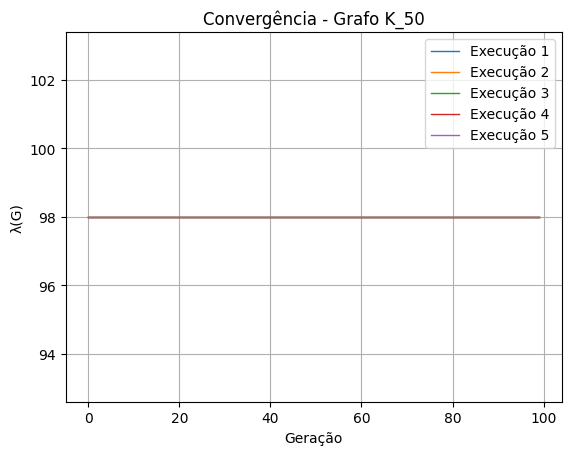
\includegraphics[width=\textwidth]{figuras/convergencia_5.png}
                \label{fig:convergencia-5}
            \end{minipage}
            \hfill
            \begin{minipage}[b]{0.48\textwidth}
                \centering
                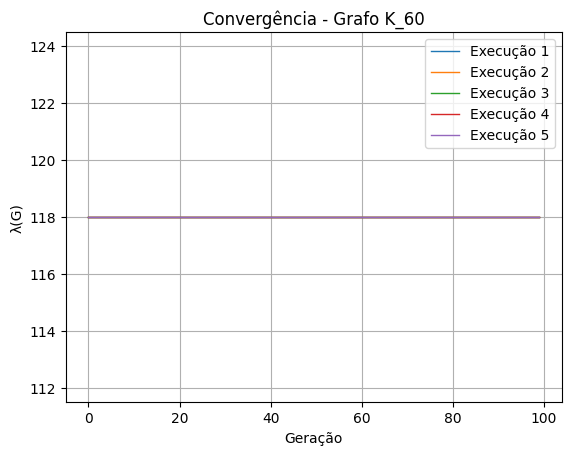
\includegraphics[width=\textwidth]{figuras/convergencia_6.png}
                \label{fig:convergencia-6}
            \end{minipage}
            
            \begin{minipage}[b]{0.48\textwidth}
                \centering
                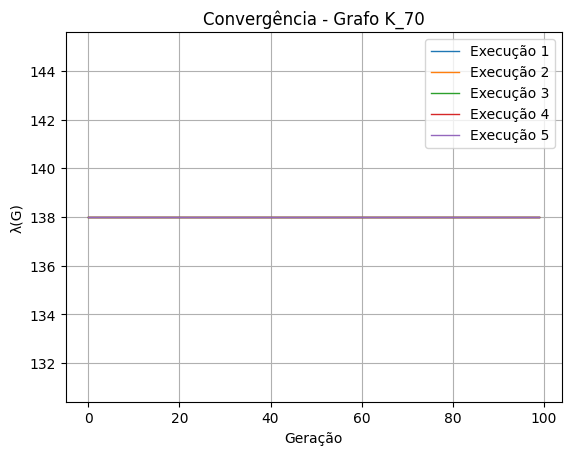
\includegraphics[width=\textwidth]{figuras/convergencia_7.png}
                \label{fig:convergencia-7}
            \end{minipage}
        \end{minipage}
    }
    \caption*{Fonte: Elaborado pelo autor.}
\end{figure}

